\documentclass[conference]{IEEEtran}

\usepackage{graphicx,url}
\usepackage{float}
\usepackage{tikz}
\usetikzlibrary{shapes, arrows, shapes.geometric}

\usepackage[brazilian]{babel}
\usepackage[utf8]{inputenc}
\usepackage[T1]{fontenc}

\graphicspath{ {../images/} }

% correct bad hyphenation here
\hyphenation{op-tical net-works semi-conduc-tor}


\begin{document}
\title{VRSnake: um Jogo de Realidade Virtual em GPGPU}


% author names and affiliations
% use a multiple column layout for up to three different
% affiliations
% \author{Adriano M. Gil\inst{1}, Eliamara Silva\inst{1}, Thiago S. Figueira\inst{1}}

% \address{Samsung Instituto de Desenvolvimento para a Informática da Amazônia
%   (SIDIA)\\
%   Manaus -- AM -- Brazil
%   \email{\{adriano.gil,eliamara.s,t.figueira\}@samsung.com}
% }

%\author{\IEEEauthorblockN{Thiago S. Figueira\IEEEauthorrefmark{1},
%Adriano M. Gil\IEEEauthorrefmark{1}}
%\IEEEauthorblockA{\IEEEauthorrefmark{1}Samsung Instituto de Desenvolvimento para a Informática da Amazônia\\
%SIDIA,\\
%Manaus -- AM -- Brazil}} 


\maketitle

% As a general rule, do not put math, special symbols or citations
% in the abstract
\begin{abstract}
Aplicações de realidade virtual são caracterizadas pela alta sensibilidade à atrasos na sincronização entre os movimentos do usuário e a respectiva renderização do mundo virtual. Uma forma de acelerar a execução da camada lógica é transportar sua implementação para GPU.  Este artigo propõe uma arquitetura de visualização baseada em um \textit{shader} parametrizado pelo variavéis de estados e movimentações dos elementos de jogo. Como exemplo dessa abordagem, implementamos uma versão do clássico jogo Snake onde todos os elementos visuais são definidos e desenhados via \textit{shader} em um único \textit{mesh}.
\end{abstract}
% no keywords


% For peerreview papers, this IEEEtran command inserts a page break and
% creates the second title. It will be ignored for other modes.
\IEEEpeerreviewmaketitle

% Reescrito
\section{Introdução} \label{sec:introduction}

% Unity e Pipeline Gráfica
O motor e editor gráfico \textit{Unity} é uma ferramenta comum para o desenvolvimento de software em realidade virtual e aumentada. Usualmente, uma aplicação \textit{unity} é constituída por cenas providas de um sistema lógico próprio que, uma vez agrupadas, formam todos os elementos pertinentes ao universo do jogo. Neste aspecto, a \textit{pipeline} gráfica rotineiramente utilizada pelas apliações e jogos \textit{unity} contempla, em linhas gerais, os seguintes passos:  a CPU (\textit{central processing unit}) transmite informações sobre os elementos gráficos à GPU (\textit{graphics processing unit}) através do estágio de aplicação, onde os \textit{assets} gráficos como modelos 3D e suas texturas são carregados na VRAM (\textit{video random access memory}), posteriormente durante o estágio de geometria, os objetos que devem ser renderizados bem como seus respectivos posicionamentos e demais informes visuais relevantes são tratados pela GPU e, em última instância, convertidos em imagem no estágio de rasterização \cite{akenine2008real}.

% Proposta
Este trabalho propõe o desenvolvimento de um jogo de realidade virtual através de uma arquitetura onde ambas as camadas lógica e de renderização gráfica sejam fundamentadas em código de GPU, o \textit{shader}. Em alusão à um clássico, o jogo \textit{snake} será recriado para os dispositivos de realidade virtual Samsung em uma aplicação \textit{unity}, diferencia-se do original na medida que o jogador controla, através do \textit{joystick}, o posicionamento do objeto coletável ao invés da serpente.

% Estrutura do artigo
Analisamos na seção \ref{sec:relatedworks} outros trabalhos que abordam jogos de realidade virtual. Um esclarecimento sobre as regras do jogo desenvolvido pode ser encontrado na seção \ref{sec:vrsnake}. A arquitetura proposta é detalhada na seção \ref{sec:architecture}. Apresenta-se como um jogo de realidade virtual pode ser renderizado em uma esfera invertida na seção \ref{sec:invertedsphere}. Em \ref{sec:agent}, comprende-se a movimentação da \textit{snake} e sua arquitetura de renderização. Resultados são discutidos na seção \ref{sec:results}. Por fim, pautam-se as conclusões e perspectivas de trabalhos futuros na seção \ref{sec:conclusion}.

% Reescreve explorando o GPUWars e estabelecer diferença entre este trabalho e o outro
\section{Trabalhos Relacionados} \label{sec:relatedworks}

\cite{GPGPUWars} mostram um jogo bidimensional de tiro com visão \textit{top-down} (de cima para baixo) que utiliza a GPU como principal fonte de processamento de todos os estados do jogo.

Contudo, aplicações em realidade virtual, tal qual a deste artigo, diferem das demais aplicações devido à necessidade de preencher o espaço tridimensional de forma a fornecer conteúdo para os 3 graus de liberdade (3DoF - \textit{3 Degrees of Freedom}) atualmente possíveis. A aplicação descrita em \cite{zund2015unfolding}, por exemplo, utiliza visão computacional para geração de uma visão panorâmica de um jogo de console em 8-bits. Rodando em um Oculus Rift DK2, o jogador é posicionado no centro do mundo e à medida que movimenta seu personagem, o mundo se desdobra ao seu redor, extendendo a visão de jogo para as quatro paredes do ambiente virtual.

% Reescrito
\section{VRSnake: Design do Jogo} \label{sec:vrsnake}
O \textit{VRSnake} é a versão em realidade virtual do clássico jogo 2D \textit{Snake}. No jogo original controlava-se a serpente na busca pelos coletáveis distribuídos pelo cenário, o \textit{VRSnake} permite ao jogador controlar o posicionamento destes objetos coletáveis, desta forma seu principal objetivo é derrotar as diversas serpentes, determinadas proceduralmente, que estão espalhadas no universo virtual. Propomos então as regras como seguem:

As serpentes buscam ininterruptamente o objeto coletável posicionado pelo jogador e seguem até o objeto pelo percurso que as manterão vivas por mais tempo, isto é, as serpentes desviam de si mesmas e das demais serpentes quando possível. Se este desvio não acontece, uma das serpentes é eliminada. Em outro aspecto, caso o objeto coletável seja capturado com sucesso, a \textit{snake} cresce em uma unidade de medida. O jogador vence a partida quando resta unicamente uma serpente.

%Reescrevendo
\section{Arquitetura de um Jogo GPGPU}
Jogos são aplicações interativas que executam três classes de ações: coleta, processamento e exibição de dados. %Arranjar referencia sobre software (algo mais abrangente) 
A coleta de dados foca em recolher dados dos dispositivos de entrada sejam eles teclado, mouse, toque ou \textit{joysticks}. O processamento abrange o reconhecimento dos dados coletados e sua devida tradução para o mundo do jogo, mas também garante o cumprimento das regras e gerenciamento do estado geral da aplicação. A exibição é o passo final, pois retorna ao jogador as consequências de seus atos de maneira sensorial. Desta forma, o \textit{VRSnake} é um jogo de realidade virtual que concentra as ações das classes de processamento e exibição na unidade gráfica de processamento (GPU - \textit{Graphics Processing Unit}), ao passo que a unidade central de processamento (CPU - \textit{Central Processing Unit}) é encarregada da entrada de dados.

Esta arquitetura foi implementada utilizando o motor gráfico \textit{Unity} através do HLSL (\textit{High Level Shading Language}) para os \textit{shaders} e CSharp como linguagem de programação de CPU (\textit{Central Processing Unit}).

De maneira mais abrangente, o jogador posiciona o objeto coletável através do \textit{joystick}, esta informação é coletada através da CPU e repassada à GPU. Esta última está responsável por guiar as serpentes até este objetivo, isto engloba decidir o melhor caminho, um que evite obstáculos, mas também envolve renderizar todos os objetivos vistos em cena.

Mais especificamente, a inteligência de movimentação da \textit{snake} é composta por uma função utilitária de avaliação de estados que analisa cada possibilidade. Em essência, a serpente sempre está buscando alcançar o coletável, por isso avalia o curso de menor distância no eixos X e Y e desde que não exista impedimentos, assume este caminho e repete o processo, conforme ilustra a função abaixo:

\begin{equation}
F(A) = R * (D + O)
\label{equation11}
\end{equation}

Onde R é um fator de randomização; D representa a distância de \textit{Manhattan} entre a posição atual e o objeto coletável; e O é um valor atribuído à existência ou não de obstáculos neste trajeto.

Para que a serpente mova-se de forma circular deve-se compreender o mapeamento UV (projeção de uma imagem 2D em uma superfície 3D) da superfície do objeto, neste caso, uma esfera. Basta verificar as extremidades para a presença da \textit{snake} e redesenhá-la no lado apropriado.

\section{Realidade Virtual}
Tendo em vista que a proposta deste artigo contempla um jogo essencialmente 2D, tal como o \textit{Snake} original, tem-se o desafio de exibir informação bidimensional em um cenário 3D de forma que tudo aconteça ao redor do usuário. Para tanto, recorreu-se à projeção cilíndrica equidistante. A solução padrão adotada na exibição de imagens equiretangulares em 360 graus é a esfera invertida, ou seja, uma esfera que tenha apenas seu lado interno renderizado, pois possibilita preencher completamente todo o campo de visão do usuário. A geração procedural de uma esfera pode seguir uma das duas abordagens abaixo:
\begin{enumerate}
  \begin{item} uma icosfera, i.e. uma esfera cujos vértices são distribuídos uniformemente; \end{item}
  \begin{item} geração de vertíces baseada em coordenadas de longitude/latitude. \end{item}
\end{enumerate}

% TODO: Refrasear texto
Para este trabalho, preferiu-se a segunda abordagem devido ao mapeamento de UV adotado ser o padrão para \textit{softwares} de modelagem na geração de esferas: vértices gerados a partir de coordenadas de longitude/latitude.

% 2 - Mapeamento de UV em uma esfera invertida
% Na figura \ref{fig:sphere_transversalsec} é exibida uma secção transversal da divisão de uma esfera em longitudes.
Na geração das posições dos vértices da esfera, se faz necessário definir uma quantidade de valores de longitude $N$, assim o tamanho angular $T$ para divisão longitudinal pode ser calculado pela equação \ref{longitudesize}.

\begin{equation}
T = \frac{2 \pi}{N}
\label{longitudesize}
\end{equation}

O tamanho angular total de uma quantidade de $i$ de valores de longitude pode ser dada pela equação \ref{longitudealpha}.

\begin{equation}
\alpha_{i} = i * T
\label{longitudealpha}
\end{equation}

% Considerando a figura \ref{fig:sphere_transversalsec}, percebe-se que
O seno e cosseno do ângulo T definem-se as posições X e Z dos pontos da esfera pertencentes a essa secção transversal da esfera. Dessa forma, supondo uma esfera de raio $R$, podemos escrever as equações \ref{x_d} e \ref{z_d}.

\begin{equation}
x_{i} = R * \sin(\alpha_{i})
\label{x_d}
\end{equation}

\begin{equation}
z_{i} = R * \cos(\alpha_{i})
\label{z_d}
\end{equation}

Em um corte longitudinal, é possível perceber que o raio $R$ de uma secção transversal varia ao longo da altura da esfera. Determina-se então um valor $K$ como o tamanho angular de um valor de latitude da esfera, dado um valor $M$ de latitudes, tal como visto na equação \ref{equation5}.

\begin{equation}
K = \frac{\pi}{M}
\label{equation5}
\end{equation}

O tamanho angular total de uma quantidade de $i$ de valores de latitude pode ser dado pela equação \ref{equation6}.

\begin{equation}
\alpha_{yi} = i * K
\label{equation6}
\end{equation}

A posição Y dos pontos da esfera, considerando raio unitário, pode ser dada pela equação \ref{equation7}.
\begin{equation}
y_{i} = \cos(\alpha_{yi})
\label{equation7}
\end{equation}

O raio $D_{yi}$ obtido em uma secção transversal na latitude $i$ é definido na equação \ref{equation8} como:
\begin{equation}
R_{yi} = \sin(\alpha_{yi})
\label{equation8}
\end{equation}

Aplicando-se a equação \ref{equation8} nas equações \ref{x_d} e \ref{z_d} obtém-se as posições X e Z dos vértices da esfera em função de suas coordenadas de longitude e latitude.

\begin{equation}
x_{i} = \sin(\alpha_{yi}) * \sin(\alpha_i)
\label{equation9}
\end{equation}

\begin{equation}
z_{i} = \sin(\alpha_{yi}) * \cos(\alpha_i)
\label{equation10}
\end{equation}

\section{Resultados} \label{sec:results}
Desenvolveu-se em realidade virtual o jogo \textit{Snake} no ambiente de desenvolvimento \textit{Unity}. Gerou-se uma aplicação \textit{android} testada no \textit{Samsung Galaxy S8} através do \textit{GearVR} com o controle de modelo ET-YO32, conforme apresentado na figura \ref{fig:vrcontroller}. A figura \ref{fig:VRPerformanceChart} abaixo ilustra a taxa de quadros no \textit{GearVR} através da ferramenta de avaliação de performance da \textit{Oculus}, o \textit{OVR Metrics Tool}:

\begin{figure}[H] \label{fig:VRPerformanceChart}
\centering
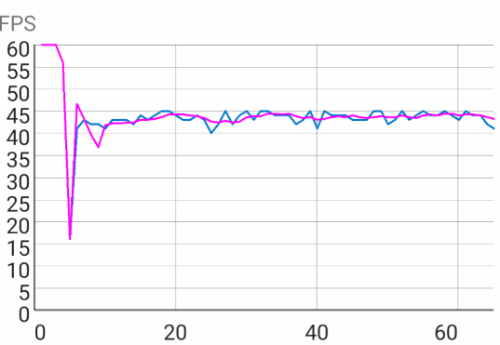
\includegraphics[scale=0.5]{VRPerformance}
\caption{Quadros-por-segundo conforme o OVR Metrics Tool executado durante o funcionamento da aplicação }
\end{figure}

A aplicação apresentou taxa média de 43.96 \textit{fps} (\textit{frames-per-second}, quadros-por-segundo), com mínima de 16 \textit{fps} e máxima de 60 \textit{fps}. Conforme representado pela figura \ref{fig:VRPerformanceChart}, a aplicação não mantém estavéis 60 \textit{fps} e isto se deve principalmente ao \textit{garbage collector}.

\section{Conclusão}\label{sec:conclusion}
% Resumo do artigo
Apresentou-se a implementação de um jogo criado segundo a arquitetura de renderização baseada em \textit{shaders} que distribui passos usualmente restritos à camada de aplicação para as demais camadas da \textit{pipeline} gráfica.

% Trabalhos Futuros
Para trabalhos futuros, há dois grandes marcos em vista: em primeiro lugar, aplicar aprendizagem de máquina ao comportamento de busca e desvio de obstáculos das serpentes afim de torná-las mais inteligentes. Em segundo lugar, otimizar e melhorar a performance, objetivando os 60 \textit{fps}. 

\bibliographystyle{IEEEtran}

% \bibliographystyle{ieeetran}
\bibliography{bare_conf}




% that's all folks
\end{document}


